\documentclass[aspectratio=169]{../latex_main/tntbeamer}  % you can pass all options of the beamer class, e.g., 'handout' or 'aspectratio=43'
\usepackage{dsfont}
\usepackage{bm}
\usepackage[english]{babel}
\usepackage[T1]{fontenc}
%\usepackage[utf8]{inputenc}
\usepackage{graphicx}
\graphicspath{ {./figures/} }
\usepackage{algorithm}
\usepackage[ruled,vlined,algo2e,linesnumbered]{algorithm2e}
\usepackage{hyperref}
\usepackage{booktabs}
\usepackage{mathtools}

\usepackage{amsmath,amssymb}

\DeclareMathOperator*{\argmax}{arg\,max}
\DeclareMathOperator*{\argmin}{arg\,min}

\usepackage{amsbsy}
\newcommand{\vect}[1]{\bm{#1}}
%\newcommand{\vect}[1]{\boldsymbol{#1}}

\usepackage{pgfplots}
\pgfplotsset{compat=1.16}
\usepackage{tikz}
\usetikzlibrary{trees} 
\usetikzlibrary{shapes.geometric}
\usetikzlibrary{positioning,shapes,shadows,arrows,calc,mindmap}
\usetikzlibrary{positioning,fadings,through}
\usetikzlibrary{decorations.pathreplacing}
\usetikzlibrary{intersections}
\pgfdeclarelayer{background}
\pgfdeclarelayer{foreground}
\pgfsetlayers{background,main,foreground}
\tikzstyle{activity}=[rectangle, draw=black, rounded corners, text centered, text width=8em]
\tikzstyle{data}=[rectangle, draw=black, text centered, text width=8em]
\tikzstyle{myarrow}=[->, thick, draw=black]

% Define the layers to draw the diagram
\pgfdeclarelayer{background}
\pgfdeclarelayer{foreground}
\pgfsetlayers{background,main,foreground}

% Requires XeLaTeX or LuaLaTeX
%\usepackage{unicode-math}

\usepackage{fontspec}
%\setsansfont{Arial}
\setsansfont{RotisSansSerifStd}[ 
Path=../latex_main/fonts/,
Extension = .otf,
UprightFont = *-Regular,  % or *-Light
BoldFont = *-ExtraBold,  % or *-Bold
ItalicFont = *-Italic
]
\setmonofont{Cascadia Mono}[
Scale=0.8
]

% scale factor adapted; mathrm font added (Benjamin Spitschan @TNT, 2021-06-01)
%\setmathfont[Scale=1.05]{Libertinus Math}
%\setmathrm[Scale=1.05]{Libertinus Math}

% other available math fonts are (not exhaustive)
% Latin Modern Math
% XITS Math
% Libertinus Math
% Asana Math
% Fira Math
% TeX Gyre Pagella Math
% TeX Gyre Bonum Math
% TeX Gyre Schola Math
% TeX Gyre Termes Math

% Literature References
\newcommand{\lit}[2]{\href{#2}{\footnotesize\color{black!60}[#1]}}

%%% Beamer Customization
%----------------------------------------------------------------------
% (Don't) Show sections in frame header. Options: 'sections', 'sections light', empty
\setbeamertemplate{headline}{empty}

% Add header logo for normal frames
\setheaderimage{
	% 
\includegraphics[height=\logoheight]{figures/TNT_darkv4.pdf}
	
\includegraphics[height=\logoheight]{../latex_main/figures/luh_logo_rgb_0_80_155.pdf}
	% 
\includegraphics[height=\logoheight]{figures/logo_tntluh.pdf}
}

% Header logo for title page
\settitleheaderimage{
	% 
\includegraphics[height=\logoheight]{figures/TNT_darkv4.pdf}
	
\includegraphics[height=\logoheight]{../latex_main/figures/luh_logo_rgb_0_80_155.pdf}
	% 
\includegraphics[height=\logoheight]{figures/logo_tntluh.pdf}
}

% Title page: tntdefault 
\setbeamertemplate{title page}[tntdefault]  % or luhstyle
% Add optional title image here
%\addtitlepageimagedefault{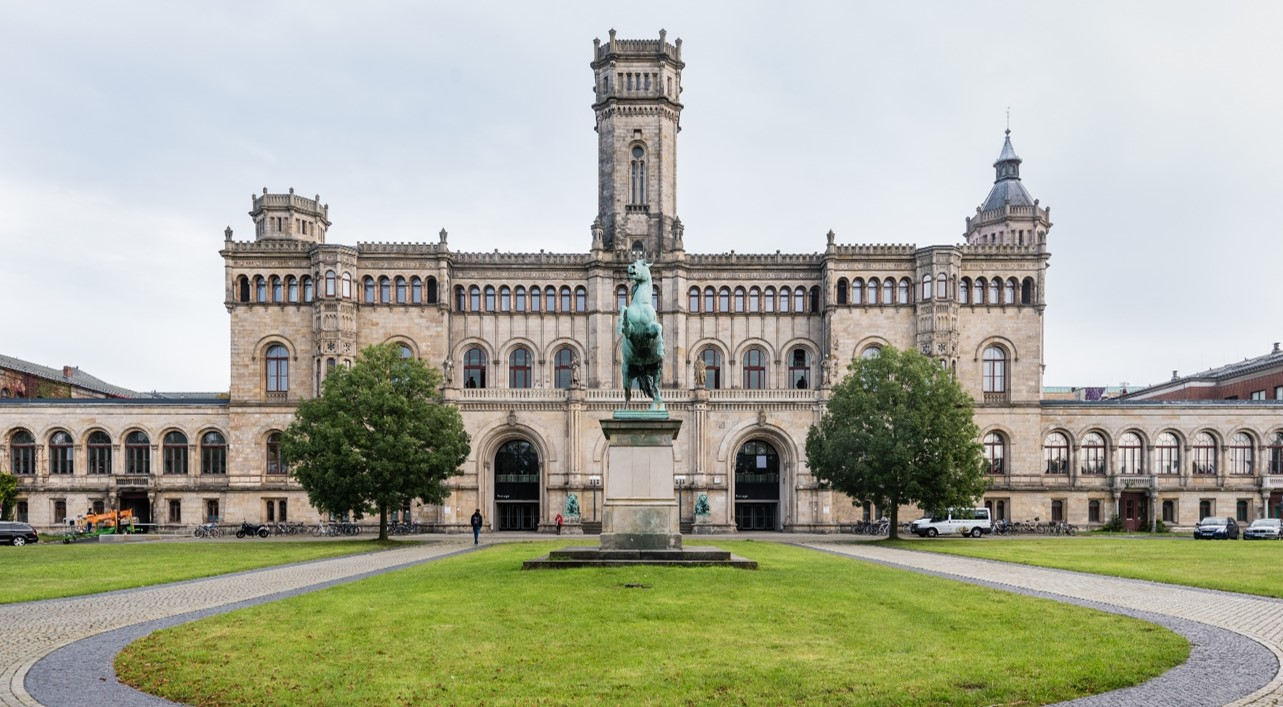
\includegraphics[width=0.65\textwidth]{figures/luh_default_presentation_title_image.jpg}}

% Title page: luhstyle
% \setbeamertemplate{title page}[luhstyle]
% % Add optional title image here
% \addtitlepageimage{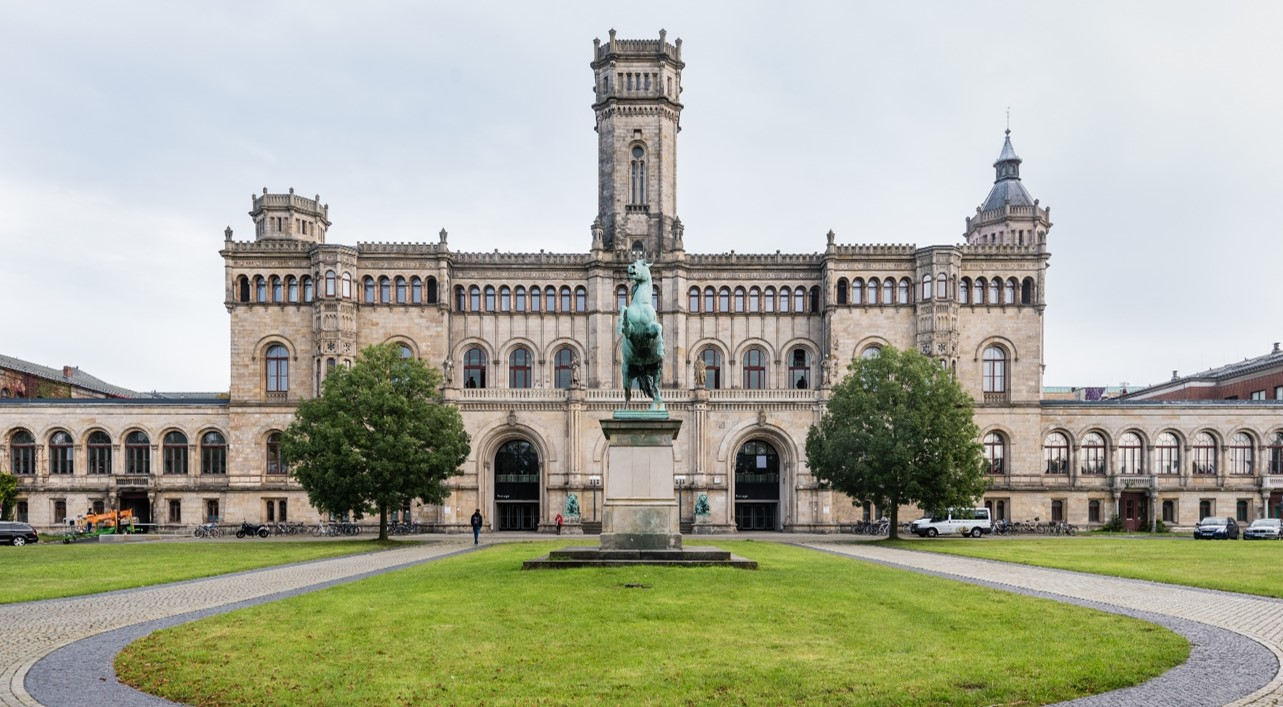
\includegraphics[width=0.75\textwidth]{figures/luh_default_presentation_title_image.jpg}}

\author[Abedjan \& Lindauer]{Ziawasch Abedjan \& Marius Lindauer\\[1em]
	
\includegraphics[height=\logoheight]{../latex_main/figures/luh_logo_rgb_0_80_155.pdf}\qquad
	
\includegraphics[height=\logoheight]{../latex_main/figures/DBIS_Kurzlogo.png}\qquad

\includegraphics[height=\logoheight]{../latex_main/figures/TNT_darkv4}\qquad

\includegraphics[height=\logoheight]{../latex_main/figures/L3S.jpg}	}
\date{Summer Term 2022; \hspace{0.5em} {
\includegraphics[height=1.5em]{../latex_main/figures/Cc-by-nc-sa_icon.svg.png}}; based on \href{https://ds100.org/fa21/}{[DS100]}
}


%%% Custom Packages
%----------------------------------------------------------------------
% Create dummy content
\usepackage{blindtext}

% Adds a frame with the current page layout. Just call \layout inside of a frame.
\usepackage{layout}


%%% Macros
%\renewcommand{\vec}[1]{\mathbf{#1}}
% \usepackage{bm}
%\let\vecb\bm

\title[Introduction]{Introduction to Data Science}
\subtitle{Logistics for the Lecture}

%\institute{}


\begin{document}
	
	\maketitle

%-----------------------------------------------------------------------------------------------------------------------------
\begin{frame}[c]{Acknowledgments}

Large parts of the material (i.e. slides, figures and exercise) were created at \href{https://ds100.org/}{[Berkeley] (University of California)}. We thank them very much for allowing us to re-use their material.

\bigskip

\alert{Warning}:
\begin{itemize}
    \item We changed material...
    \item We condensed it...
    \item We extended it...
    \item We fixed it...
\end{itemize}


\end{frame}
%-----------------------------------------------------------------------


%-----------------------------------------------------------------------------------------------------------------------------
\begin{frame}[c]{Goals of the Lecture}

You will be able to \ldots
\begin{enumerate}
  \item \alert{identify} steps needed to apply data science
  \item \alert{explain} different data processing steps required in data science
  \item \alert{choose} a promising combination of approaches to build data science pipelines
  \item \alert{evaluate} data science pipelines on different datasets
  \item \alert{visualize} data and results in data science
  \item \alert{apply} data science to new tasks at hand
\end{enumerate}

\end{frame}
%-----------------------------------------------------------------------
%----------------------------------------------------------------------
\begin{frame}[c]{Course Overview}

\begin{itemize} 
    \item Motivation [Abedjan \& Lindauer] % today: April 25th
	\item Data Sampling and Probability [Abedjan] % May 2nd
	\item Data Preprocessing [Abedjan] % May 9th
	\item Visualization [Lindauer] % May 16 th
	\item Intro to Modelling [Abedjan] % 
	\item Simple Linear Regression + Ordinary Least Squares [Lindauer] % May 30th
	\item Feature Engineering [Abedjan] % June 13th (June 6th is Pentecost)
	\item Bias and Variance [Lindauer] % June 20th 
	\item Evaluation, Regularization and AutoML [Lindauer] % June 27th
	\item Classification [Lindauer] % July 4th
	\item Inference for Modelling [Abedjan] % July 11th
	\item Conclusion \& Ethics [Abedjan] % July 18th --> that's ICML week and afterwards is AutoML-Conf --> @Ziawasch: could you please take care of this session alone?
\end{itemize}


\end{frame}
%----------------------------------------------------------------------
%----------------------------------------------------------------------
\begin{frame}[c]{Course Format}

\begin{itemize}
	\item Concepts \& details
	\begin{itemize}
	  \item We provide sufficient details s.t. you can understand and use the techniques
	  \item We highly recommend that you dig deeper and read additional material to become a real expert
	\end{itemize}
	\smallskip
	\item ``Classic'' lecture
	\begin{itemize}
	  \item 1 Slot lecture + 1 slot guided exercise
	\end{itemize}
	\smallskip
	\item Practical exercises and home works
	\begin{itemize}
	  \item implement it, use it and play with it!
	\end{itemize}
\end{itemize}

\end{frame}
%----------------------------------------------------------------------
%----------------------------------------------------------------------
\begin{frame}[c]{Team}

\begin{columns}[T]



\column{0.2\textwidth}
\centering
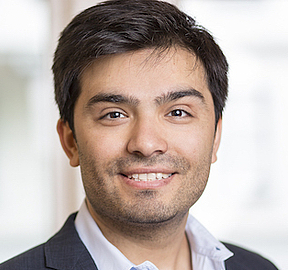
\includegraphics[height=8em]{./figures/zia}

Prof. Dr.\\ Ziawasch Abedjan

\column{0.2\textwidth}
\centering
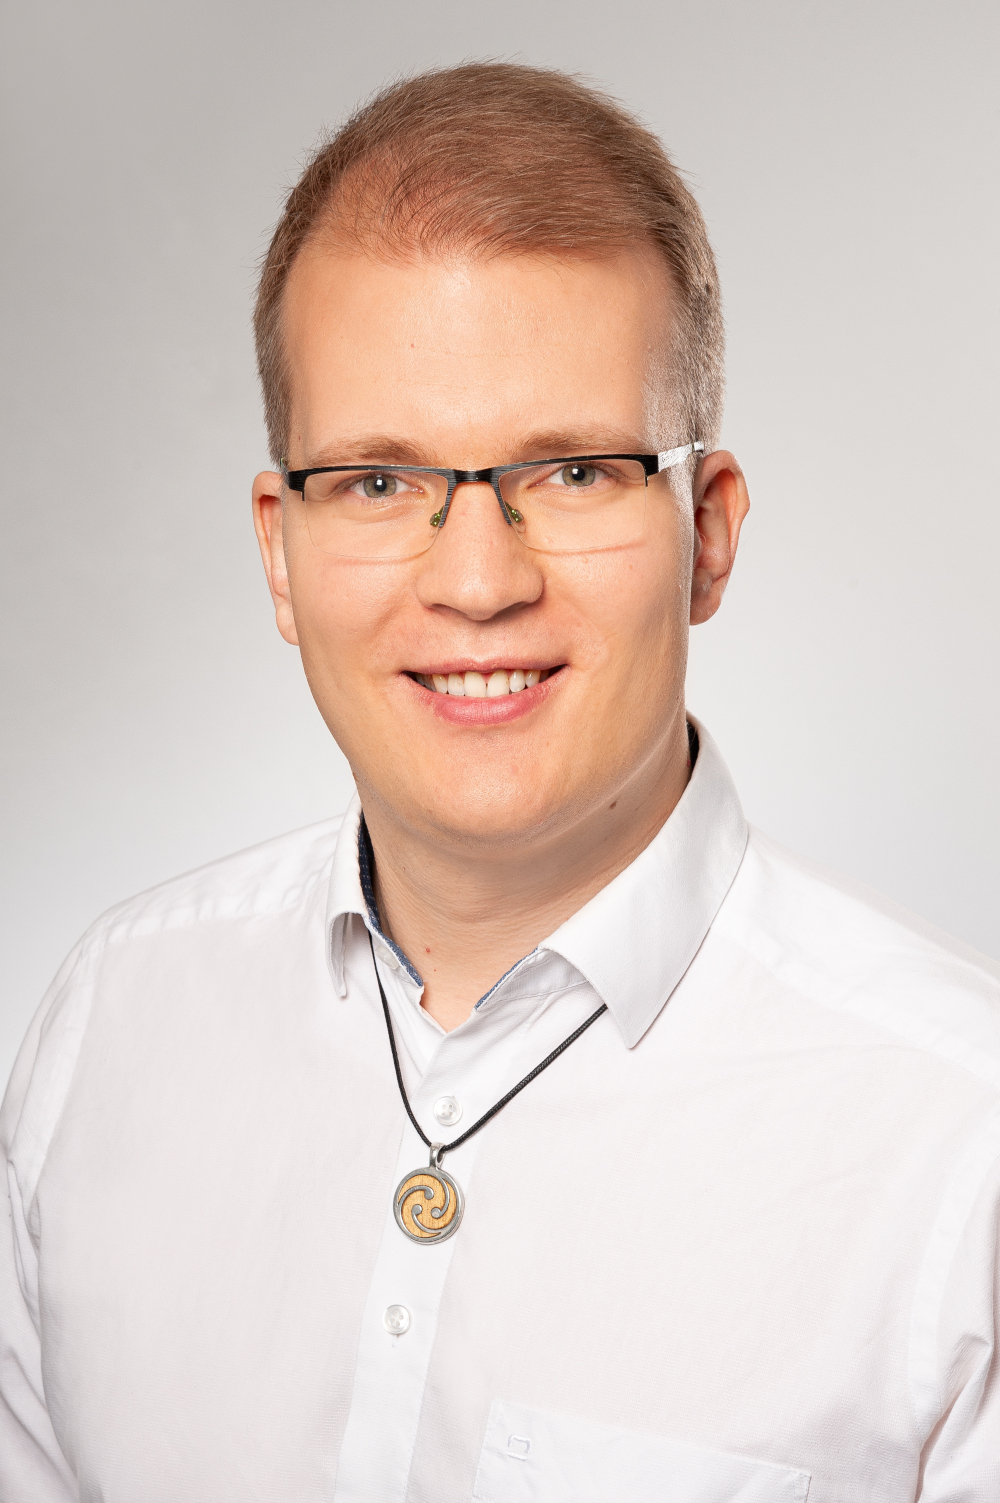
\includegraphics[height=8em]{./figures/Lindauer_Marius_004small.jpg}

Prof. Dr.\\ Marius Lindauer

\column{0.2\textwidth}
\centering
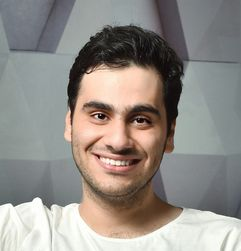
\includegraphics[height=8em]{./figures/mahdi}

Mahdi Esmailoghli\\

\column{0.2\textwidth}
\centering
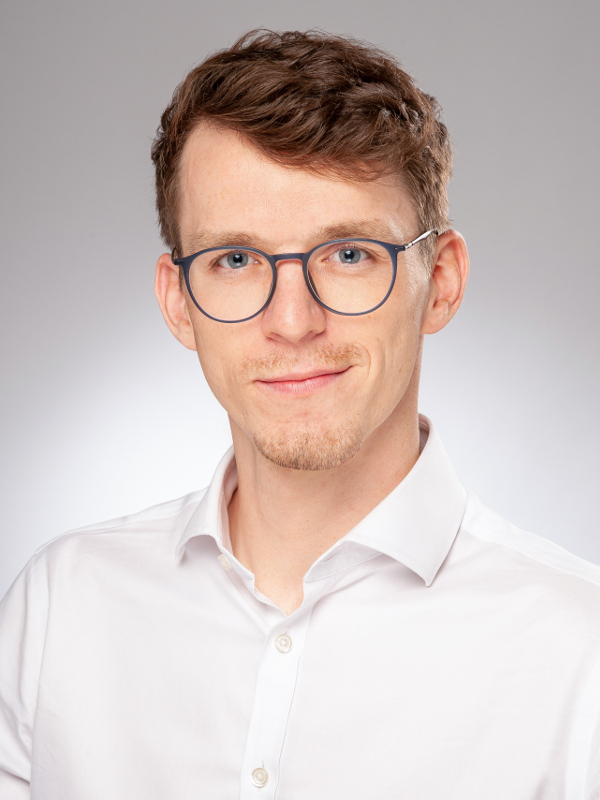
\includegraphics[height=8em]{./figures/tim}

Tim Ruhkopf\\

\end{columns}

\end{frame}
%----------------------------------------------------------------------
% %----------------------------------------------------------------------
% \begin{frame}[c]{Why Videos?}

% \begin{itemize}
%   \item Advantages of videos:
%   \begin{itemize}
%       \item Neither YOUTUBE nor NETFLIX VIDEOS!
%       \item Watch it whenever (wherever) you want
%       \item Watch it at your own speed
%       \begin{itemize}
%           \item[$\leadsto$] Stop it if you need time to think about it
%       \end{itemize}
%       \item Go back and watch it again, if you missed or forgot something
%       \item Annotate questions on the fly %(e.g., using the Miro boards)
%       \item After each video ($\sim$10-20min), you can take a break and\\ think about what you learned in this video (and whether you understood it)
%   \end{itemize}
%   \medskip
%   \pause
%   \item Risks and challenges:
%   \begin{itemize}
%       \item You have to be self-disciplined 
%       \item You have to wait with your questions until our meetings
%       \begin{itemize}
%           \item[$\leadsto$] Use our chat to discuss with your peers
%       \end{itemize}
%   \end{itemize}
% \end{itemize}

% \end{frame}
% %-----------------------------------------------------------------------
%----------------------------------------------------------------------
\begin{frame}[c]{Organization (Exercises \& Home Work)}

\begin{itemize}
  \item Every week new exercise sheet
  \begin{itemize}
      \item Exercise focus is aligned with lectures
      \item Do the exercises in the exercise sessions (Thursdays at 11:00am s.t.)
      %\item Watch videos and start to directly work on exercise 
      %\item[$\leadsto$] \alert{Deadline one day after the live session: Wednesday at 23:59}
  \end{itemize}
  \item Most exercises will be practical, i.e., you have to implement something
  \begin{itemize}
    \item Expected work load: 1.5h each week
  \end{itemize}
  \item Team work highly recommended, e.g. team size of 3!
  \item Home work every 3 weeks, i.e. 4 times overall
  \begin{itemize}
      \item You can get \alert{5\% as bonus points} for the final exam
      \item You need 66\% of all homework points to get the bonus points\\
      $\leadsto$ either you get all the bonus points or none at all
  \end{itemize}
  \pause
  \item Don't cheat (incl. plagiarism)
  \begin{itemize}
    \item First time cheating: $0$ points for exercise / homework
    \item Second time cheating: failing the course
  \end{itemize}
  \pause
  \item Homework is not mandatory\\ \alert{BUT: quite unlikely that you will pass the course without doing them}
  \pause
\end{itemize}

\end{frame}
%-----------------------------------------------------------------------
% %----------------------------------------------------------------------
% \begin{frame}[c]{Live Discussion}

% \begin{itemize}
%   \item Every week at Tuesday: 09:30am (s.t) - 11:30am\\ 
%   \item Room: Multimedia Room at L3S (15th floor, Appelstr. 9a)
%   \pause
%   \item Warning: Does not replace watching the recorded lecture videos!
%   \pause
%   \smallskip
%   \item Components:
%   \begin{enumerate}
%       \item You can ask anything related to the recent lecture videos or exercises
%       \item Break-out to discuss questions in small groups (if number of attendees to allow this)
%       \pause
%       \item Q\&A regarding the exercise
%       \pause
%       \item Interactive quiz where you can check whether you understood the main points
%   \end{enumerate}
%   \pause
%   \medskip
%   \item No recordings of the live sessions
% \end{itemize}

% \end{frame}
% %-----------------------------------------------------------------------
%----------------------------------------------------------------------
\begin{frame}[c]{Get in Touch with Us}

\begin{itemize}
  \item Lecture session every Monday (14:00am s.t.) and exercise session every Thursday (11:00 am s.t.)
  \item \alert{Use the forum in StudIP for all kind of questions}
  \item Don't send us emails
  \begin{itemize}
      \item[$\leadsto$] Only in case of emergencies
  \end{itemize}
\end{itemize}

\end{frame}
%-----------------------------------------------------------------------
%----------------------------------------------------------------------
\begin{frame}[c]{Requirements for Attending}

\begin{itemize}
    \item Basics in \alert{Statistics} (mandatory)
    \begin{itemize}
        \item We will cover many concepts, but you need a basic understanding of the underlying math.
    \end{itemize}
  \item Programming in \alert{Python} (mandatory)
  \begin{itemize}
    \item all exercises will require that you implement something in~Python 
    \item We will show you basics at the beginning in the exercises.\\ However if you never used Python before, it could get quite hard for you.
  \end{itemize}
  \item \alert{English} (mandatory)
    \begin{itemize}
    \item You can ask us any question also in German. However, we will reply in English. So, you need to understand us ;-)
  \end{itemize}
\end{itemize}

\end{frame}
%-----------------------------------------------------------------------
%----------------------------------------------------------------------
\begin{frame}[c]{Final Project Exam -- Tentative Plan!}

\begin{itemize}
  \item Written Exam
  \item Show us that you understood the concepts
  \item Be a master of all the algorithms we showed you
  \item Be able to read and check code
  \item ...
\end{itemize}

\end{frame}
%----------------------------------------------------------------------
%----------------------------------------------------------------------
\begin{frame}[c]{Additional Resources}

\begin{itemize}
  \item There are also awesome online courses (MOOCs), teaching you many concepts
  \begin{itemize}
      \item Data science is such a big field
      \item Don't expect that you will learn everything in a single lecture / course\\ $\leadsto$ there might be parts you can only learn in our lecture (e.g., AutoML)
      \item \href{https://www.coursera.org/specializations/data-science-python}{Applied Data Science with Python Specialization} by the University of Michigan
      \item \href{https://www.coursera.org/learn/machine-learning/home/welcome}{Machine Learning} by Andrew NG
  \end{itemize}
  \item \href{https://www.kaggle.com/}{Kaggle} for online competitions, datasets and code
  \begin{itemize}
      \item If you can become a grant master at Kaggle, you have very good chances for job offers
      \item Participate in competitions, look for help in forums, polish your skills!
      \item \href{https://github.com/abhishekkrthakur/approachingalmost}{Approaching (almost) any machine learning problem}\\ by Abhishek Thakur (first 4x Grant Master at Kaggle)
  \end{itemize}
\end{itemize}

\end{frame}
%----------------------------------------------------------------------
%----------------------------------------------------------------------
\begin{frame}[c]{Opportunities and Risks}

``Introduction to Data Science'' is a basic lecture.\\ It is the first time we teach it at the Leibniz University Hannover.

\bigskip
\pause

Opportunities:
\begin{itemize}
  \item Get all the basics you need to do your own first data science projects
  \item Perfect foundation for other AI courses at the LUH (most of them in the masters; see next slide)
\end{itemize}

\medskip

Risks:
\begin{itemize}
  \item You will find some typos and issues in the slides;\\ please tell us if you find something
  \item We will not cover deep neural networks
\end{itemize}

\medskip
$\to$ Give us some feedback and we will improve the course!

\end{frame}
%-----------------------------------------------------------------------
%----------------------------------------------------------------------
\begin{frame}[c]{AI@LUH}

\centering
\vspace{-1.3cm}
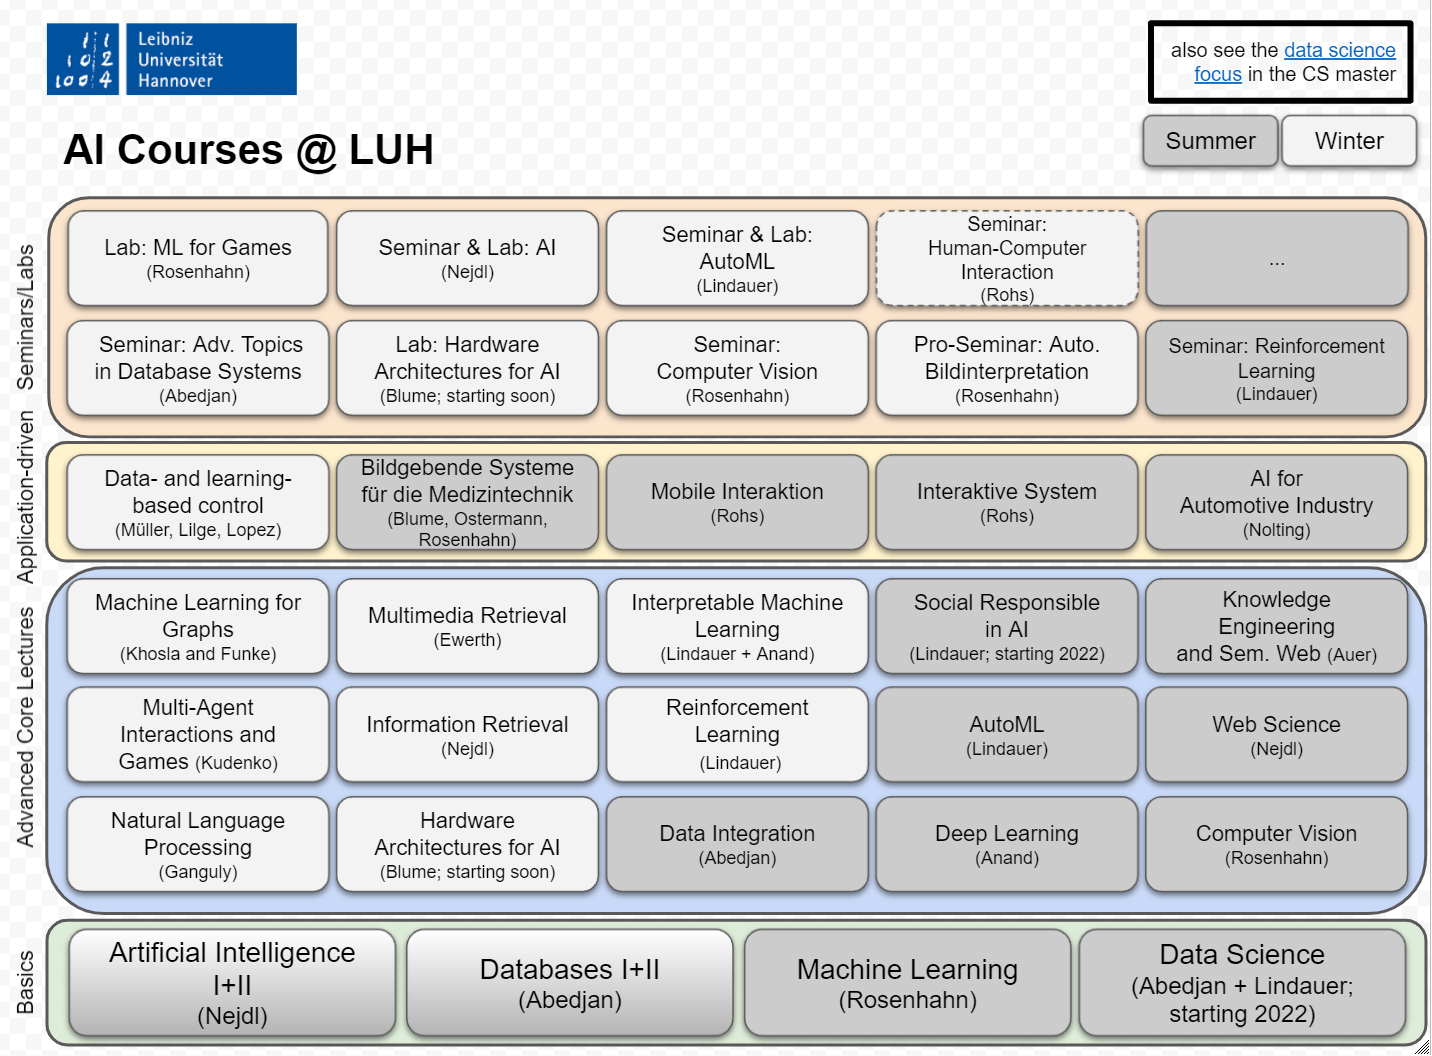
\includegraphics[width=0.75\textwidth]{./figures/ai_luh.PNG}

\end{frame}
%-----------------------------------------------------------------------
%----------------------------------------------------------------------
\begin{frame}[c]{Introduce yourself}


\begin{center}
\huge
    Introduce yourself!
\end{center}

\begin{itemize}
    \item What drives you for being here?
    \item What interests you in data science?
    \item Do you already have hands-on experience in data science?
    \item Are you looking for team members for exercises and home works?
\end{itemize}

\end{frame}
%-----------------------------------------------------------------------

% \end{frame}

\begin{frame}[c]{}

\centering
\huge
Questions?

\end{frame}

	
\end{document}
